%!TEX root = ../report.tex
\chapter{Implementation}\label{ch:implementation}

% TODO @all add introduction to implementation
\lipsum[2-4]

\section{Libraries}\label{sec:libraries}
% TODO rename this chapter to make clear that the libraries are self-developed
% TODO @all add introduction to libraries
% -> why libraries?
% -> advantages?
% -> disadvantages?

\subsection{Persistence}\label{subsec:persistence}

% TODO @joernneumeyer & @mauritsvanderzee
% TODO add link to npm

\subsection{Transport}\label{subsec:transport}
% TODO @joernneumeyer & @mauritsvanderzee
% TODO add link to npm

\subsection{Utilities}\label{subsec:utilities}
% TODO @joernneumeyer & @mauritsvanderzee
% TODO add link to npm

\section{Frontend}\label{sec:frontend}

\subsection{Services}\label{subsec:services}

The following part of the dossier will describe the different services which have been developed during the time of the project.
This will include a description of each service, followed by an REST API specification.

\subsubsection{API Service}\label{subsubsec:api-service}

The API service is a rather small service located in the desktop client.
The service is responsible for managing the global state of all relevant API information in the desktop application.
In the current state of development this includes the following information

\begin{itemize}
    \item hostname - the hostname of the server (e.g. trale.org)
    \item port - the default port on which the service is listening for incoming connections (default: 8086)
    \item the remote endpoint - a constructed string for building a connection to the server (e.g.\ http://trale.org:8086)
    \item trale port - the default port on which the service is listening for encrypted messages (default: 8087)
\end{itemize}

Further, the service provides several helper methods for retrieving and updating the remote endpoint as well as several
getters and setters for all above mentioned attributes.

\subsubsection{Auth Service}\label{subsubsec:auth-service}
The auth service is responsible for managing authentication related tasks such as login, logout, registration and
minor helper functions (e.g.\ forgot password).

\paragraph{Login function}
The login takes a username and a password as parameters and executes a post request to the remote endpoint specified in
the \textbf{\hyperref[subsubsec:api-service]{API service}}.
On a successful login a token will be provided for future authentication, otherwise an error stating 'Invalid
credentials - Status code 400' will be returned.

% TODO @joernneumeyer maybe add register / logout etc. here as well? refactor code? not in auth service yet

Due to the mentioned responsibilities, this service is only injected in authentication related components.

\subsubsection{Contact Service}\label{subsubsec:contact-service}

The contact service is responsible for managing all contact related tasks and corresponding state management.
It owns a contact array holding all contacts for the currently logged-in user.
On application startup the contact service will load all contacts from drive by utilizing the
\textbf{\hyperref[subsubsec:crypto-storage-service]{Crypto Storage Service}}.

Besides providing a loading wrapper for retrieving encrypted contacts from the drive it also manages actions such as
adding contacts, updating contacts or fetching the latest message of all contacts to display those in the contact list.

Lastly, the contact service provides a function to load the actual chat of a specific contact with the currently
logged-in user.

% TODO @joernneumeyer any additional remarks / information to be added?

\subsubsection{Debug Service?}
% TODO @joernneumeyer & @mauritsvanderzee
% @joernneumeyer shall we include debug service?

\subsubsection{Crypto Storage Service}
% TODO @joernneumeyer & @mauritsvanderzee

\subsubsection{Key Registry Service}
% TODO @joernneumeyer & @mauritsvanderzee

\subsubsection{Titp Service}
% TODO @joernneumeyer & @mauritsvanderzee

\subsubsection{Util Service}
% TODO @mauritsvanderzee

\subsection{Components}

\section{Backend}

\subsection{Database Connections}

\subsection{Services}

\subsubsection{Authentication Service}
% TODO @joernneumeyer

\subsubsection{File Service}
% TODO @all shall we just briefly mention that this might be a service for future features / development

\subsubsection{Identity Service}
\label{subsubsec:identitySer}
% TODO @joernneumeyer

\subsubsection{Settings Service}
\label{subsubsec:settingsSer}
% TODO @maltecastner & tobiasjansen
The Settings service provides an interface to the admin panel frontend and carries out the settings to the other services.
This service was developed in parallel to the admin panel frontend. %TODO @maltecastner insert reference to component, once it has been added
First only the for the UI necessary functionality would be added, later on the actual functionality was added (e.g.\ that users can actually be reported for the report reasons added in the settings)
As visible from the use case diagram~\ref{fig:ucd} the Settings service carries out a few tasks by itself whilst forwarding
certain other request to the identity ~\ref{subsubsec:identitySer} and the reporting~\ref{subsubsec:reportingSer} service.
The use cases and their descriptions can be found on in the online documentation.

\begin{figure}[!ht]
    \centering
    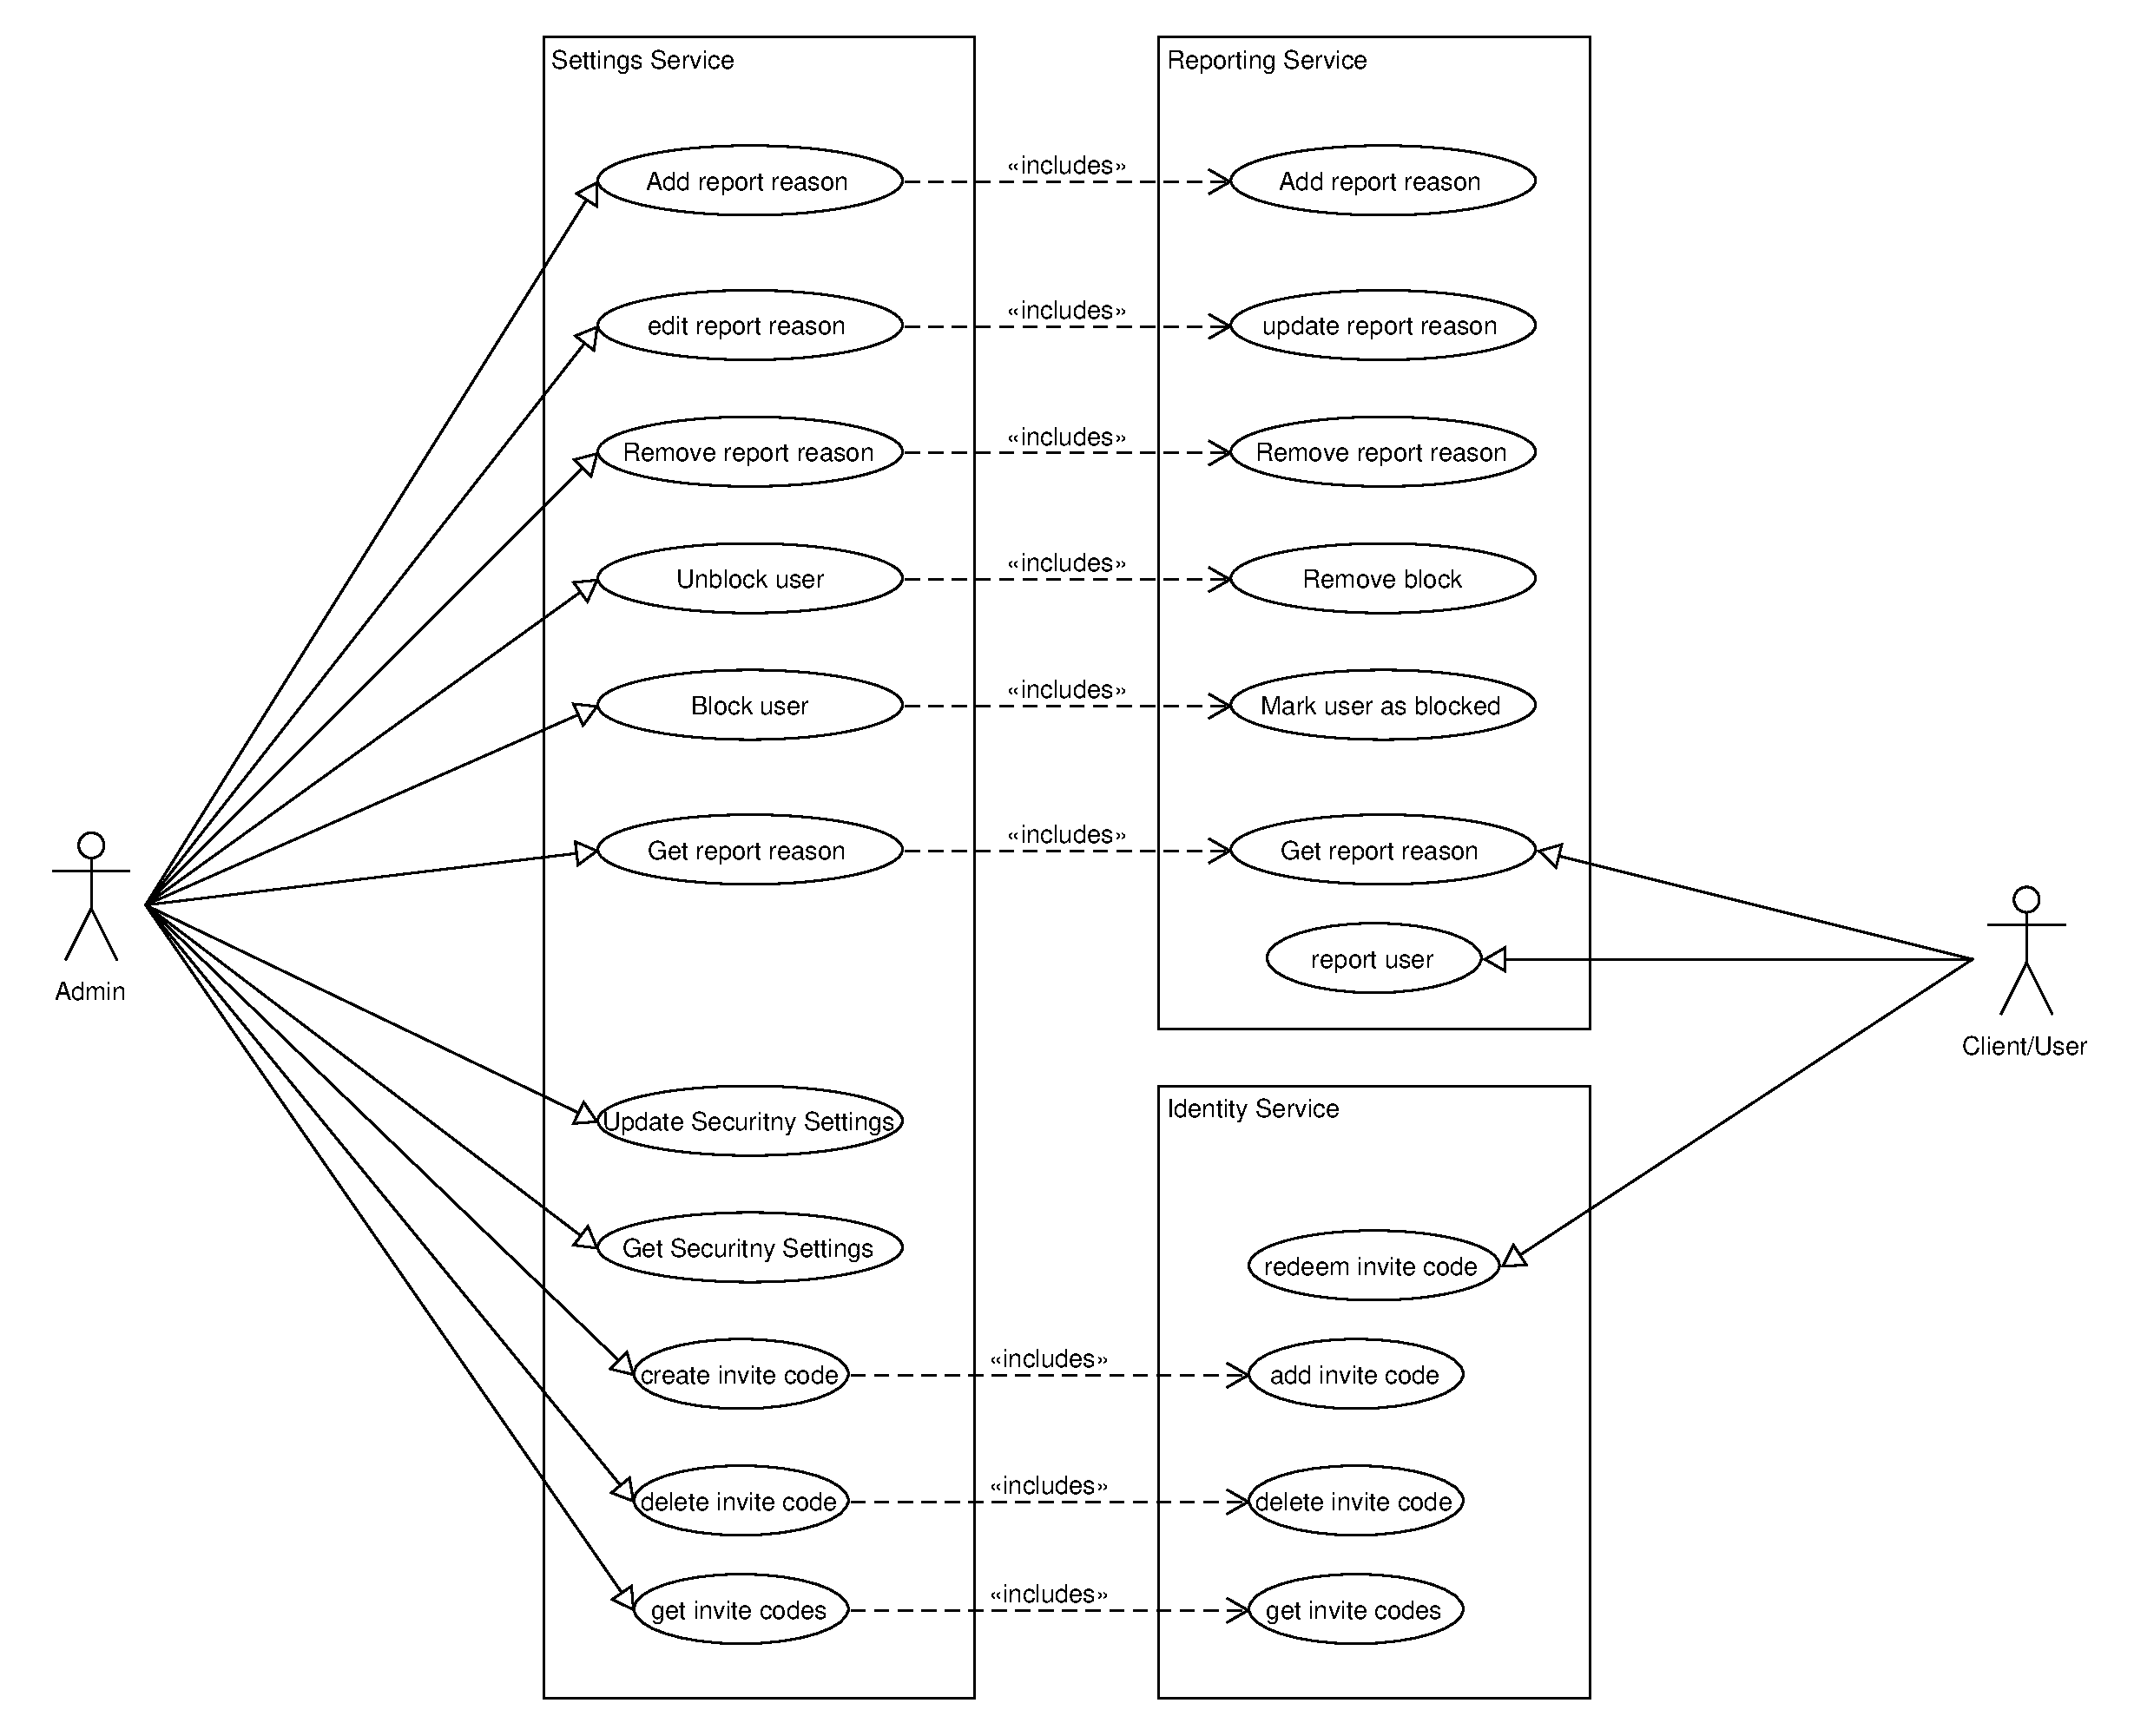
\includegraphics[width=1.0\textwidth]{./images/UseCaseDiagramAdminPanel.pdf}
    \caption{Use case diagram of the admin panel showing responsibility of each AP service}
    \label{fig:ucd}
\end{figure}

\paragraph{Rest interface}
The settings service provides the following rest endpoints:

\begin{verbatim}
GET: /settings/report-reason
\end{verbatim}

Returns all report reasons as a JSON array.

\begin{verbatim}
POST: /settings/report-reason
body:
{
"reason": "some reason",
"max_report_violations": 5
}
\end{verbatim}
adds a new report reason.

\begin{verbatim}
PUT: /settings/report-reason
body:
{
"id": 123,
"reason": "some reason",
"max_report_violations": 5
}
\end{verbatim}
Edits an existing report reason.


\begin{verbatim}
DELETE: /settings/report-reason
headers:
- "id": 123
\end{verbatim}

Deletes a report reason with an id that is provided as a header.

\begin{verbatim}
GET: /settings/security
\end{verbatim}

returns the current security settings.

\begin{verbatim}
PUT: /settings/security
body:
{
    "two_factor_auth": {
    "on" : true,
    "phone": false,
    "email": true
},
    "confirmed_emails_only": true,
    "individual_pwd_req": {
    "on": true,
    "upper_case": true,
    "number": true,
    "special_char": true,
    "reg_ex": false,
    "reg_ex_string": "[]"
},
    "inv_only": {
        "on": false,
        "inv_only_by_adm": false
    }
}
\end{verbatim}
Edits the security settings.
The new settings are provided in body.

##Example Add Report reason
\begin{figure}[!ht]
    \centering
    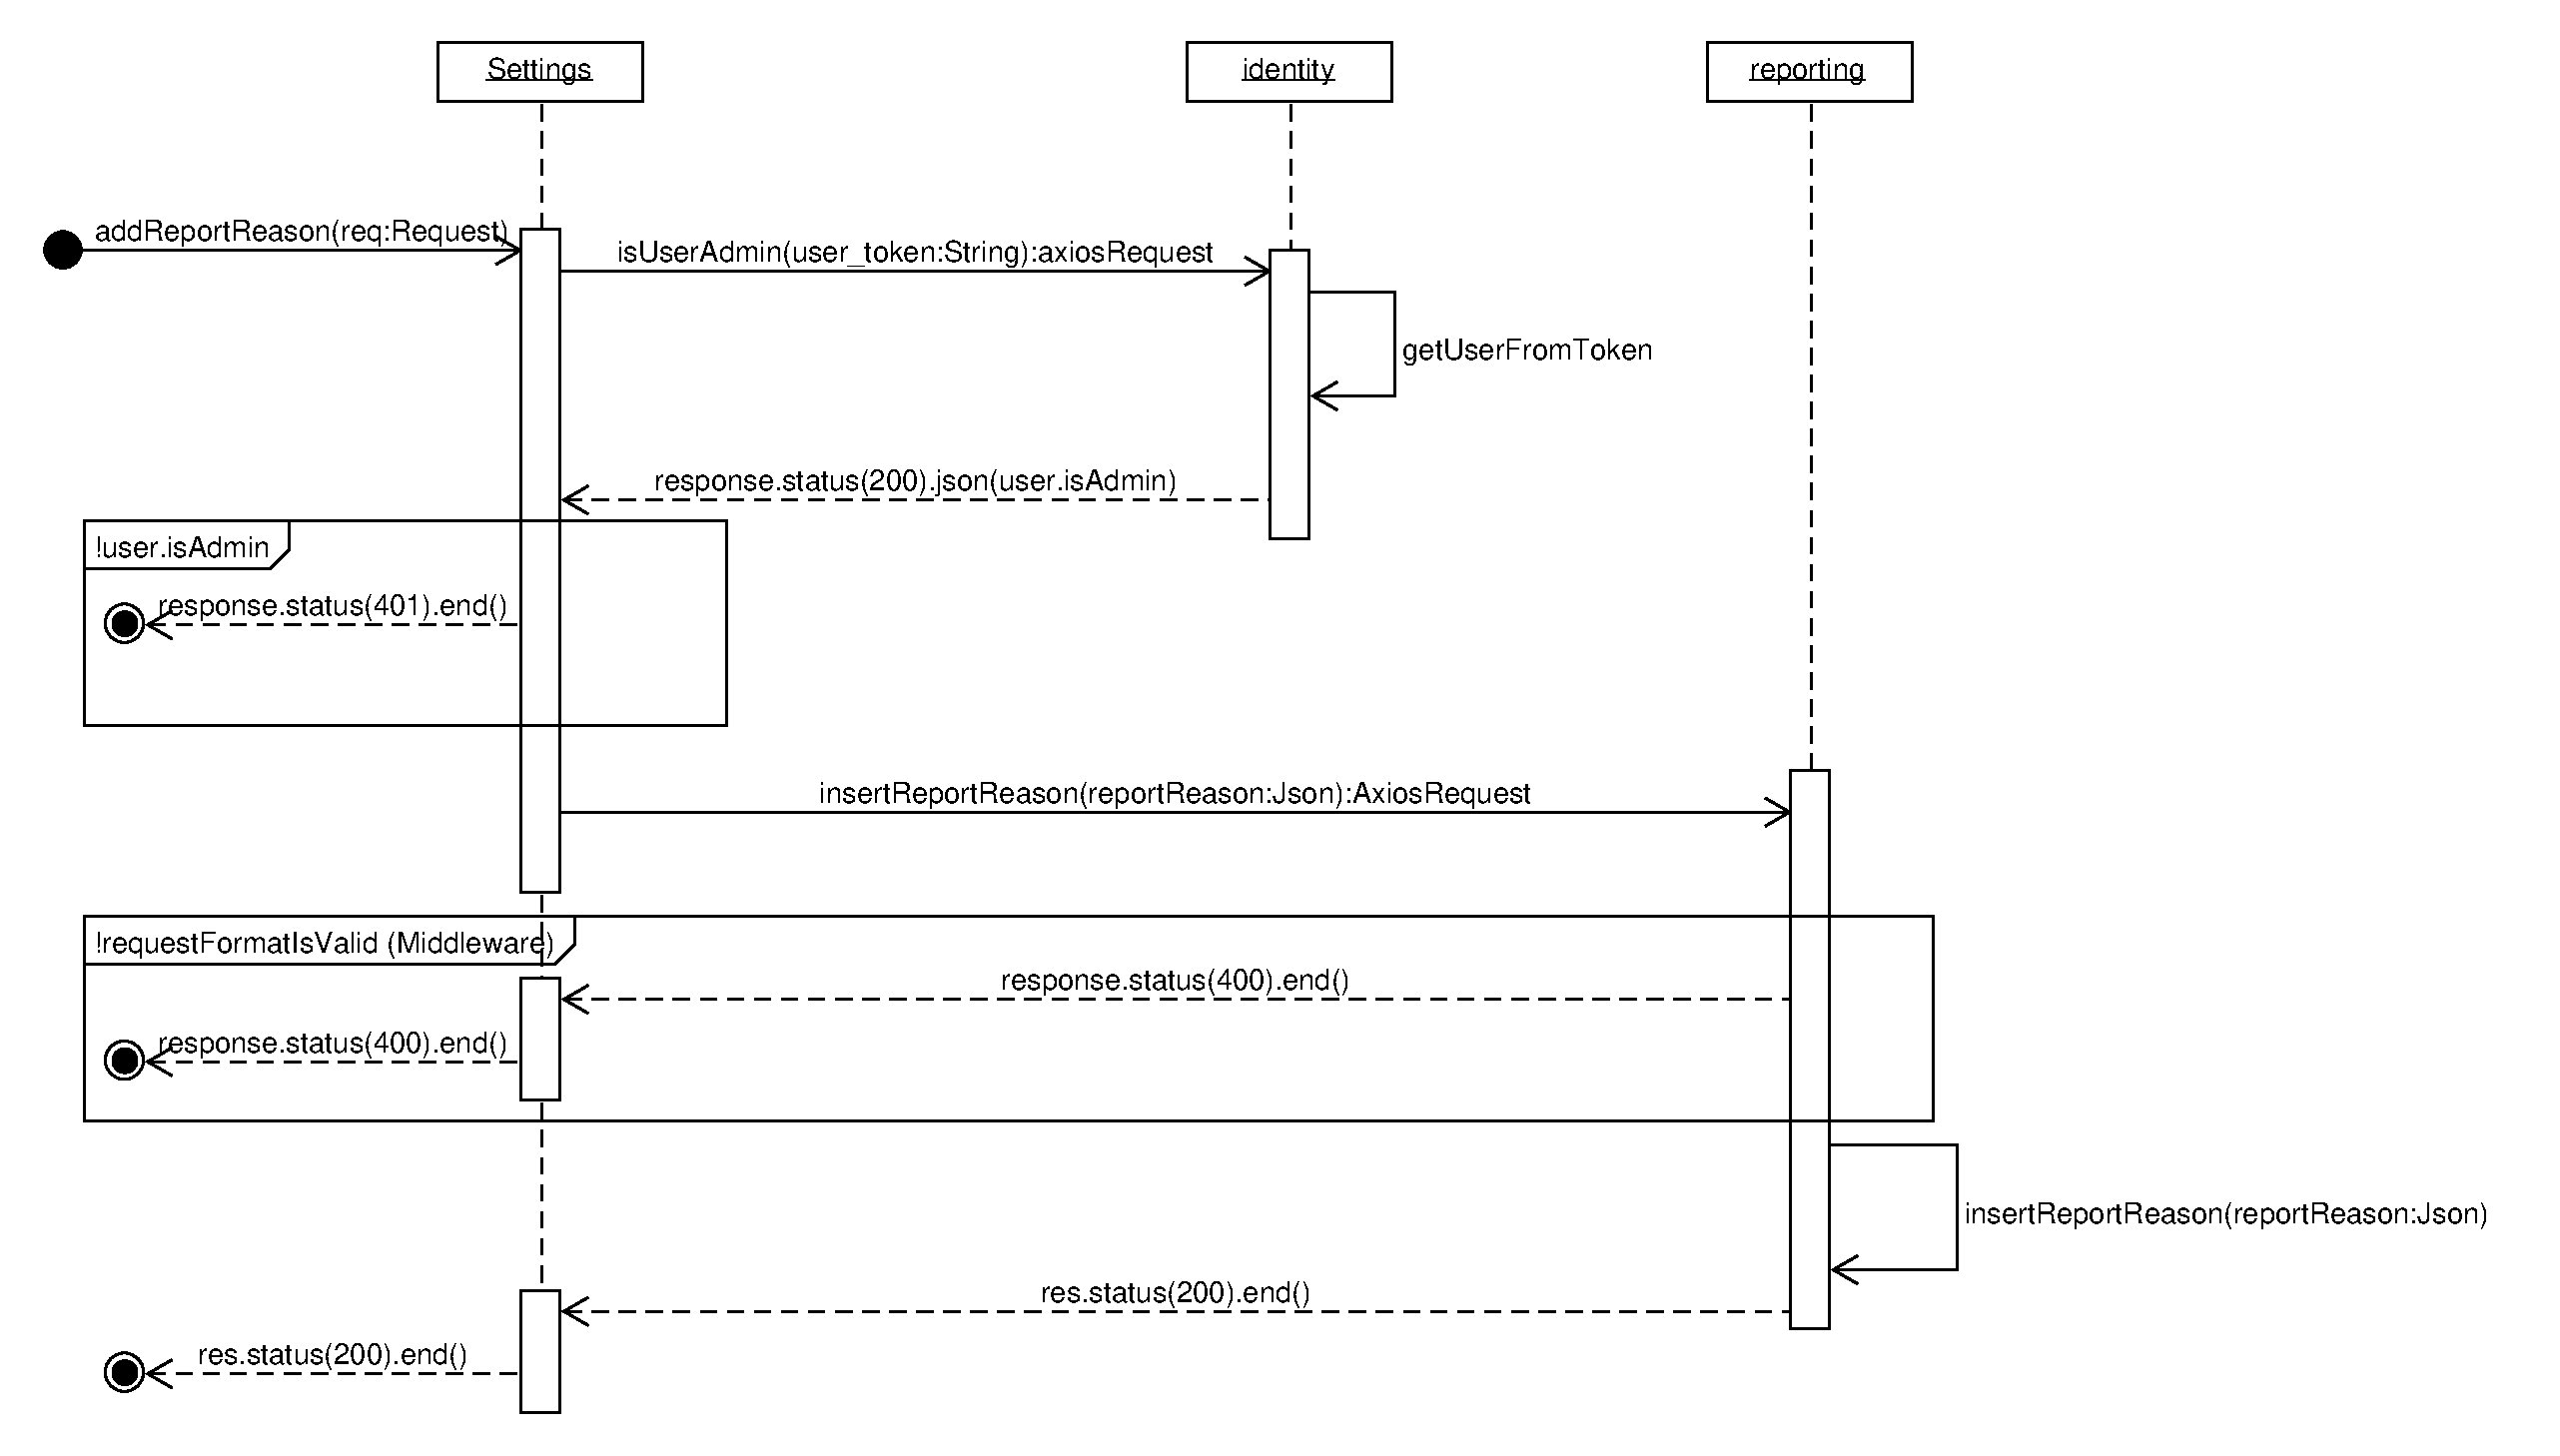
\includegraphics[width=1.0\textwidth]{./images/SequenceDiagram_AddReportReason.pdf}
    \caption{Use case diagram of the admin panel showing responsibility of each AP service}
    \label{fig:addReportReason}
\end{figure}
The sequence diagram~\ref{fig:addReportReason} shows an example of the communication of the settings service with the aforementioned services.
The event is triggered by a request from the client.
Firstly the settings service will be verifying the identity of the sender by checking at the identity service, if the user who sent out the request is in fact an administrator.
Then the request will e forwarded to the reporting service. Here it will be checked if the request format is valid. Should this not be the case, the reporting service will return an error (status 400).
Otherwise the reason will be added in the reporting database, which will then be returned to the settings service, who will then let the client know by response that the insertion was a success.
This way each service has a clearly defined task.

\subsubsection{Reporting Service}
\label{subsubsec:reportingSer}
% TODO @maltecastner & tobiasjansen
The reporting service handles the reporting system.
This includes administrative tasks like managing for which reasons users can be reported, as well as the reporting system itself (reporting users and banning them).
The administrative tasks, like adding new report reasons, manually blocking and unblocking users, can be done via the
settings service~\ref{subsubsec:settingsSer}.
This service was added in the later stages of the project.
First the entire reporting was handled via the settings service~\ref{subsubsec:settingsSer}, however it was decided that the reporting itseslf should possess its own service.
Therefore it was necessarry to outsource the report related functionality from the settings service to the reporiting service

\paragraph{Rest Interface}
\begin{verbatim}
POST: /report-reasons
body:
{
    "reason": "some reason",
    "max_report_violations": 5
}
\end{verbatim}
Adds a new report reason returning the id of the added report reason.

\begin{verbatim}
PUT: /report-reasons
body:
{
    "id": 12
    "reason": "some reason",
    "max_report_violations": 5
}
\end{verbatim}
Edits a report reason by the "id" key and returns the edited reason.

\begin{verbatim}
GET: /report-reasons
\end{verbatim}
Returns all existing report reasons as JSON array

\begin{verbatim}
DELETE: /report-reasons
headers
    - id: 12
\end{verbatim}
Deletes a report reason by id which is provided in the header of the request.
Returns the id of the deleted request in its body.

\begin{verbatim}
Headers:
    - user_token
Body:
{
    "username": "userHashOfUserBeingReported",
    "reason_id": 123
}
\end{verbatim}
Reports a user based of the report reason and the users username hash.
A user can only be reported by a the same user for the same reason after 15 minutes to prevent spamming.
Otherwise the report will be processed by the backend and the user set to "blocked" should he exceed the maximum report violation counter.